Die Erarbeitung des Lösungsansatzes wird anhand der Erkenntnisse
aus den theoretischen Grundlagen des Projektmanagements aus Kapitel \ref{chap:theorie_teil},
der gewonnenen Informationen aus der Analyse des IST-Zustandes aus Kapitel \ref{chap:analyse} 
und des Branchenvergleiches aus Kapitel \ref{chap:branchenvergleich} erstellt.
Das Resultat ist ein überarbeiteter Projektablauf, der die definierten Anforderungen 
aus Kapitel \ref{chap:anforderungen} erfüllt.

\section{Projektablauf}
Die nachfolgende Grafik \ref{pic:01_projektablauf} zeigt den neuen Projektablauf 
mit einer Aufteilung in vier Hauptabschnitte. Jedem Abschnitt wurden Resultate
hinzugefügt, die während dieser Phase erarbeitet oder durchgeführt werden sollen.

\begin{figure}[htbp]
\begin{center}
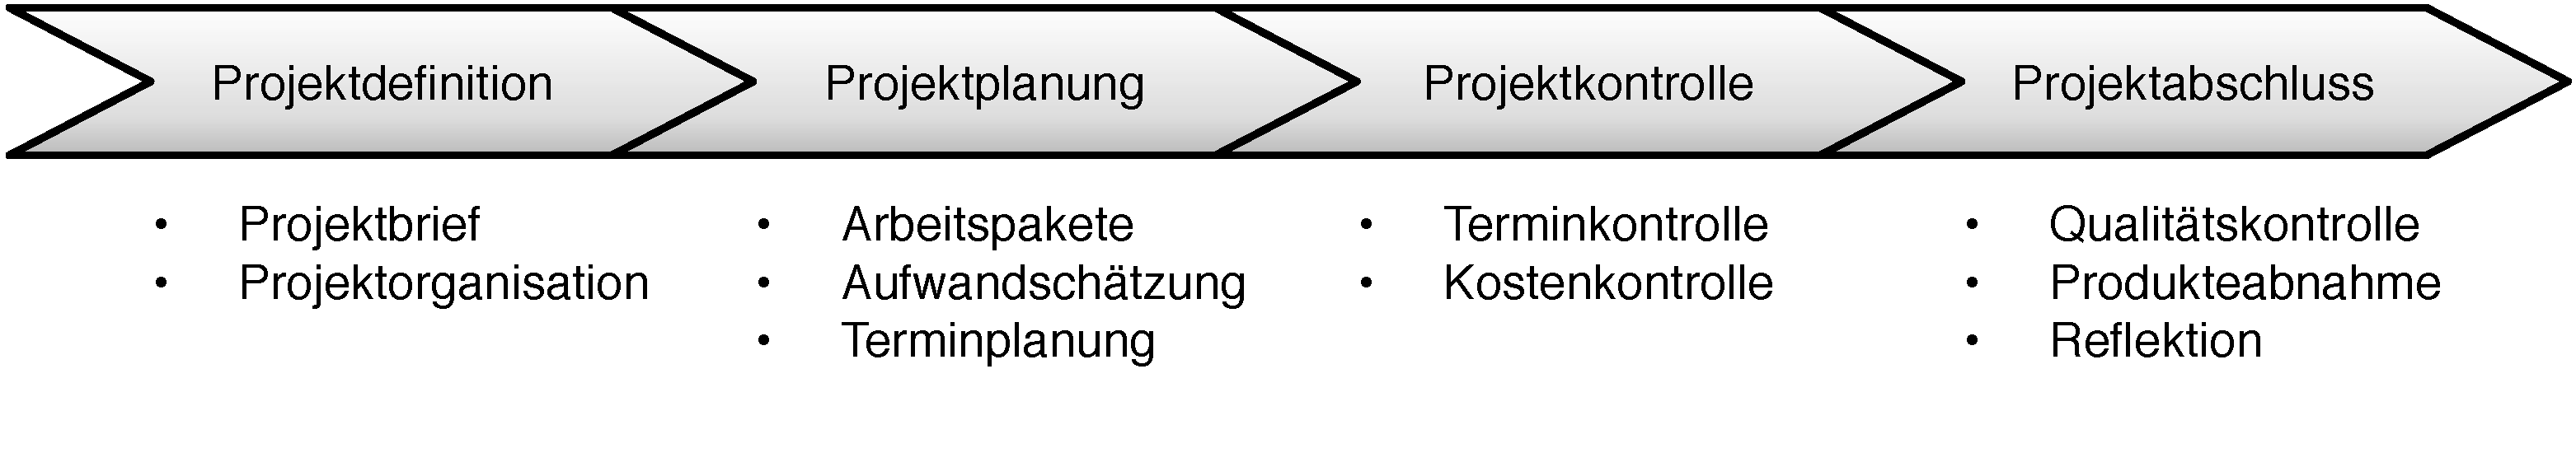
\includegraphics[width=0.99\textwidth,angle=0]{./bilder/loesung/01_projektablauf.pdf}
\caption[Aufteilung des Projektablaufes mit Resultaten]{Aufteilung des Projektablaufes mit Resultaten\footnotemark}
\label{pic:01_projektablauf}
\end{center}
\end{figure}
\footnotetext{Eigene Darstellung}

In den folgenden Kapiteln wird einzeln auf die vier Hauptabschnitte und deren
Resultate eingegangen. Es wird aufgezeigt, wie die jeweils erwarteten Resultate 
erarbeitet werden sollen.

Zusätzlich werden die Stellen hervorgehoben, wo der Einsatz und die Verwendung 
von Instrumenten sinnvoll ist. Die Wahl dieser Instrumente wird später in einem
separaten Kapitel \ref{chap:instrumentenwahl} behandelt. Zum besseren Verständnis
wird an den jeweiligen Stellen das nötige Instrument mit einer fortlaufenden
Nummer (\textbf{AI}n) versehen. So kann darauf im separaten Kapitel wieder Bezug 
genommen werden.

\newcounter{icounter}
\subsection{Projektdefinition}
In der Grafik \ref{pic:02_01_projektdefinition} ist der Ablauf der Projektdefinition 
ersichtlich. Die potenziellen Projekte (\textbf{0}) gelangen weiterhin zu den
Partnern (\textbf{1.1}), die entscheiden ob ein Projekt angenommen werden soll
oder nicht (\textbf{1.2}). Im Falle einer Absage, wird das dem Kunden von einem
Partner mitgeteilt (\textbf{2.1} bis \textbf{2.3}).

Wird das Projekt angenommen, bestimmen die Partner einen Hauptverantwortlichen
Partner und einen Verantwortlichen Projektleiter (\textbf{3.1}). Der Projektleiter
erstellt darauf den Projektbrief (\textbf{3.2}) und kümmert sich danach um
die Projektorganisation (\textbf{3.3}).

\begin{figure}[htbp]
\begin{center}
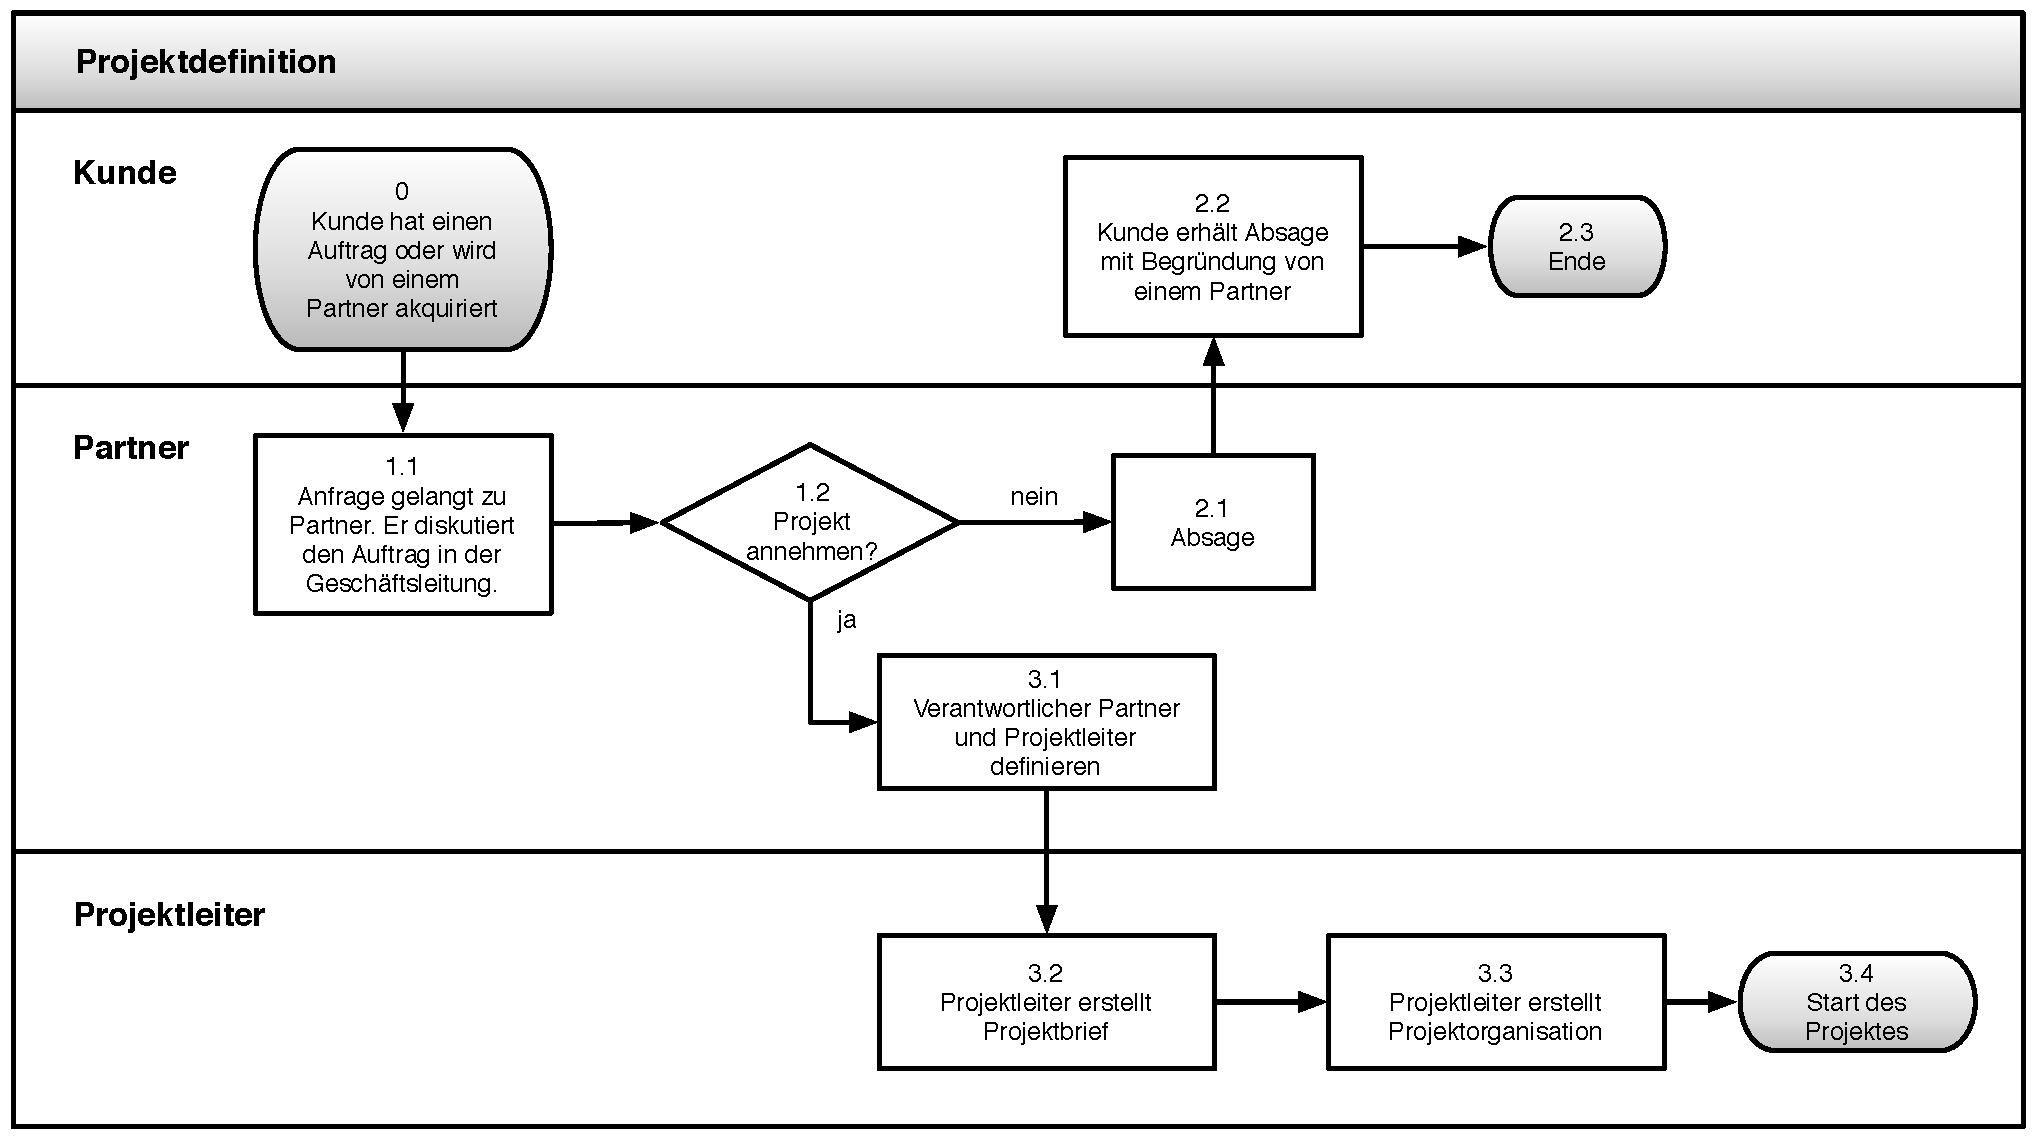
\includegraphics[width=0.99\textwidth,angle=0]{./bilder/loesung/02_01_projektdefinition.pdf}
\caption[Ablauf der Projektdefinitionsphase]{Ablauf der Projektdefinitionsphase\footnotemark}
\label{pic:02_01_projektdefinition}
\end{center}
\end{figure}
\footnotetext{Eigene Darstellung}

\subsubsection{Projektbrief}
Der Projektbrief beinhaltet alle wichtigen Angaben zum Projekt. Der Projektbrief 
sollte eine A4 Seite nicht überschreiten, da er allen Mitarbeitern im Projekt 
möglichst einfach und klar den Kern des Projektes häher bringen soll.

In der nachfolgenden Tabelle \ref{tab:projektbrief} sind
die Elemente des Projektbriefs dargestellt und zusätzlich beschrieben.

\begin{longtable}{lp{10cm}}
    \toprule \textbf{Element} & \textbf{Beschreibung} \\
    \midrule Kunde, Kontaktperson &
        Namen des Kunden und Kontaktperson \\
    \midrule Projekt &
        Namen des Projektes \\
    \midrule Datum &
        Erstellungsdatum des Projektbriefs \\
    \midrule Hintergrund &
        Beschreibung der Ausgangslage. Was müssen wir wissen? \\
    \midrule Aufgabe &
        Was möchte der Kunde von uns? \\
    \midrule Ziel &
        Was wollen wir mit dem Projekt erreichen? \\
    \midrule Zielgruppe &
        Mit wem kommunizieren wir? Wer ist die Zielgruppe? \\
    \midrule Botschaft und USP &
        Was muss das Produkt kommunizieren und was ist das Verkaufsargument? \\
    \midrule Tonalität &
        Wie kommunizieren wir das Produkt? \\
    \midrule Vorgaben, Obligatorisches &
        Was muss verwendet und beachtet werden? Gibt es Vorgaben? \\
    \bottomrule
    \caption[Aufbau eines Projektbriefs]{Aufbau eines Projektbriefs\footnotemark}
    \label{tab:projektbrief}
\end{longtable}
\footnotetext{Eigene Darstellung}

Den Projektbrief kann der Projektleiter in Zusammenarbeit mit dem verantwortlichen 
Partner erarbeiten. Sobald dieser erstellt ist, sollte klar sein, was für 
Ressourcen für das Projekt benötigt werden und der Projektleiter kann sich um 
die Projektorganisation kümmern.

\subsubsection{Projektorganisation}
Beim Aufbau der Projektorganisation macht sich der Projektleiter Gedanken dazu,
was für Ressourcen er für die Umsetzung des Projektes benötigt. Dazu wählt er,
wenn nötig unter Absprache mit dem verantwortlichen Partner, die geeigneten 
Ressourcen. Dies ergibt dann, wie in der Grafik \ref{pic:03_projektorganisation} 
abgebildet, eine Auftrags-Projektorganisation.

\clearpage

\begin{figure}[htbp]
\begin{center}
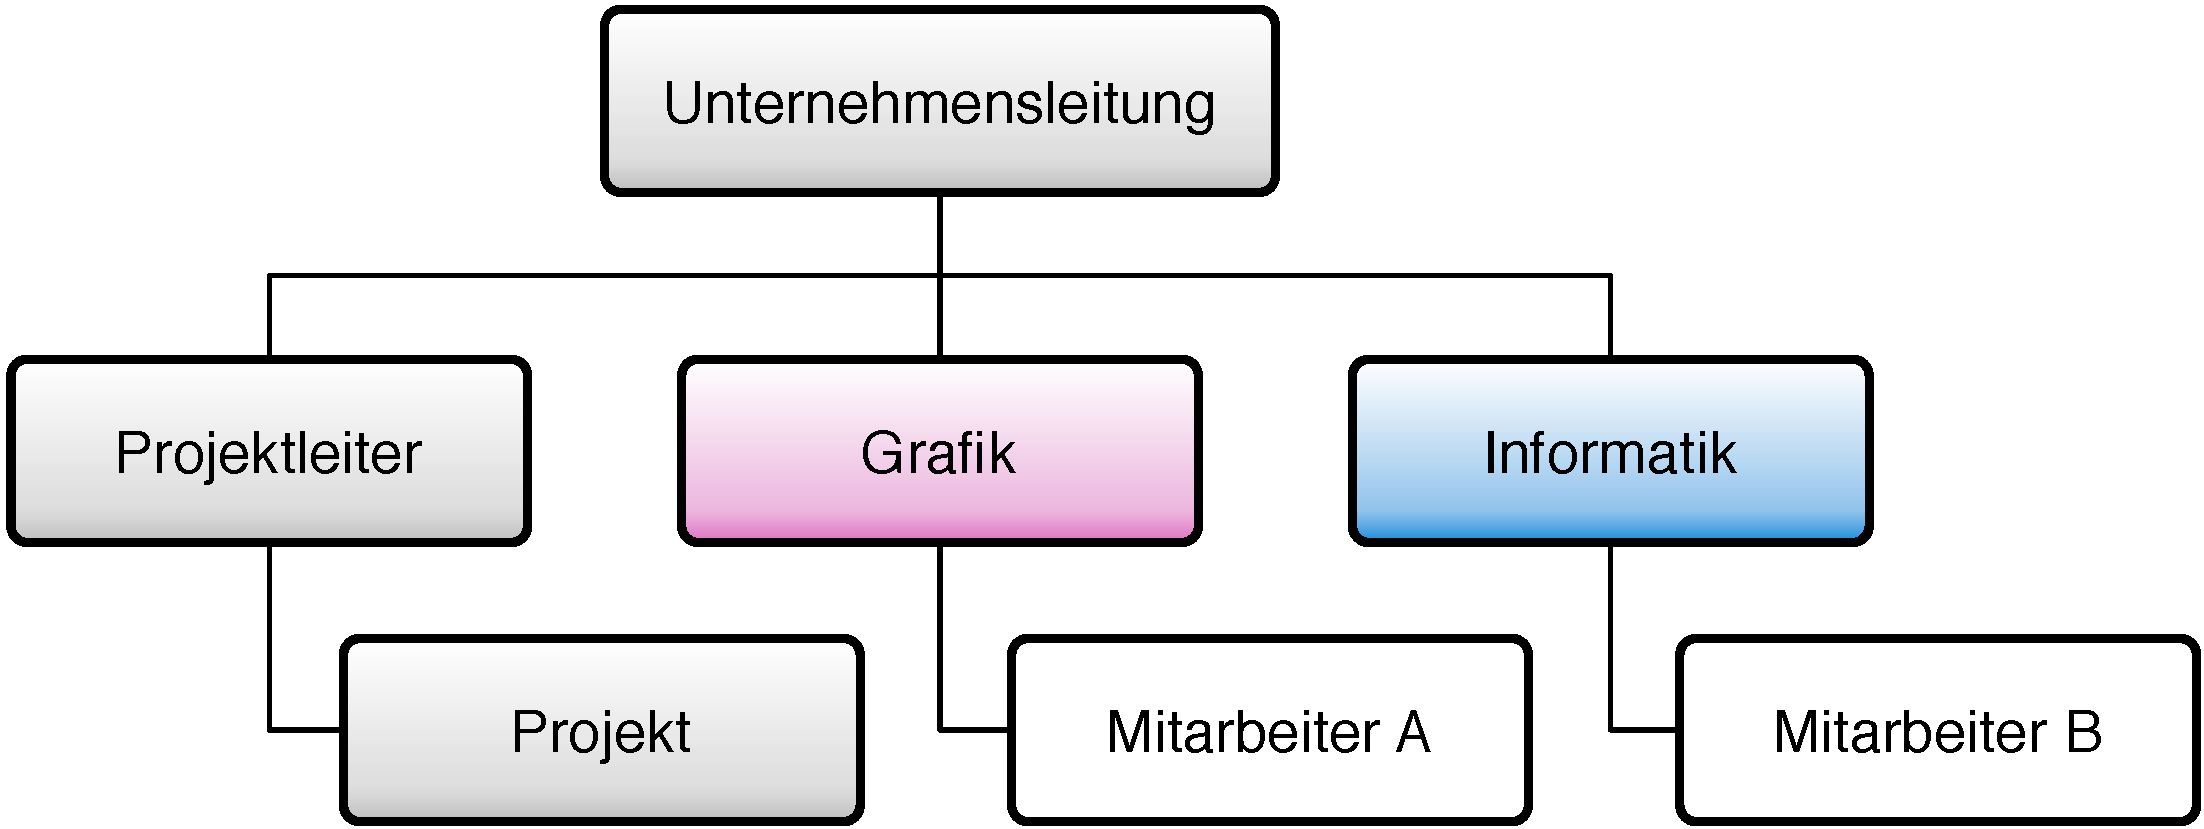
\includegraphics[width=0.7\textwidth,angle=0]{./bilder/loesung/03_projektorganisation.pdf}
\caption[Auftrags-Projektorganisation]{Auftrags-Projektorganisation\footnotemark}
\label{pic:03_projektorganisation}
\end{center}
\end{figure}
\footnotetext{Eigene Darstellung}

Der Projektleiter sucht sich die geeignetsten Mitarbeiter aus, um eine saubere 
Projektplanung erstellen zu können. Gewisse Mitarbeiter können auch nur für die 
Projektplanung, also zum Beispiel als Experten für die Aufwandsschätzung, 
eingeplant werden. Es ist wichtig, dass zu diesem Zeitpunkt noch keine 
Ressourcenplanung erstellt wird. Ist zu diesem Zeitpunkt auch nicht möglich,
da noch keine Projektplanung existiert.

Der Projektleiter eröffnet nun das Projekt im Projektmanagement Tool 
(\textbf{\addtocounter{icounter}{1}AI\arabic{icounter}}) mit einer fortlaufenden
Projektnummer und einer eindeutigen Projektbezeichnung, damit die Aufwände
der Projektplanung bereits auf das Projekt rapportiert werden können.

\subsection{Projektplanung}
In der Grafik \ref{pic:02_02_projektplanung} ist der Ablauf der Projektplanung 
ersichtlich. Als erstes überprüft und sammelt der Projektleiter alle nötigen
Unterlagen, die zur Planung des Projektes notwendig sind (\textbf{3.5}). Falls
noch Unterlagen oder Informationen von Seiten des Kunden fehlen (\textbf{3.6})
fordert er diese beim Kunden ein (\textbf{4.1}). Sobald alle Informationen
vorhanden sind, werden die Arbeitspakete zusammen mit den Mitarbeitern und 
Experten erstellt (\textbf{5.1}). Sind die Arbeitspakete definierte, werden
diese ebenfalls vom Projektleiter in Zusammenarbeit mit den Mitarbeitern und
Experten geschätzt (\textbf{5.2}). Alle Mitarbeiter müssen die hierfür aufgewendete
Zeit auf das Projekt rapportieren (\textbf{\addtocounter{icounter}{1}AI\arabic{icounter}}).

Der Projektleiter erstellt danach die Offerte und macht einen Vorschlag mit
realistischen Timings und Meilensteinen (\textbf{5.3}). Die Offerte bespricht er
mit dem verantwortlichen Partner (\textbf{5.4}). Der Partner wiederum bespricht
danach die Offerte mit dem Kunden (\textbf{5.6}). Wenn weitere Änderungen oder
Anpassungen nötig sind (\textbf{5.7}), nimmt diese der Projektleiter vor. Sobald
die Offerte vom Kunden abgesegnet ist, wird mit der Durchführung des Projektes
begonnen (\textbf{6.1}).

\clearpage

\begin{figure}[htbp]
\begin{center}
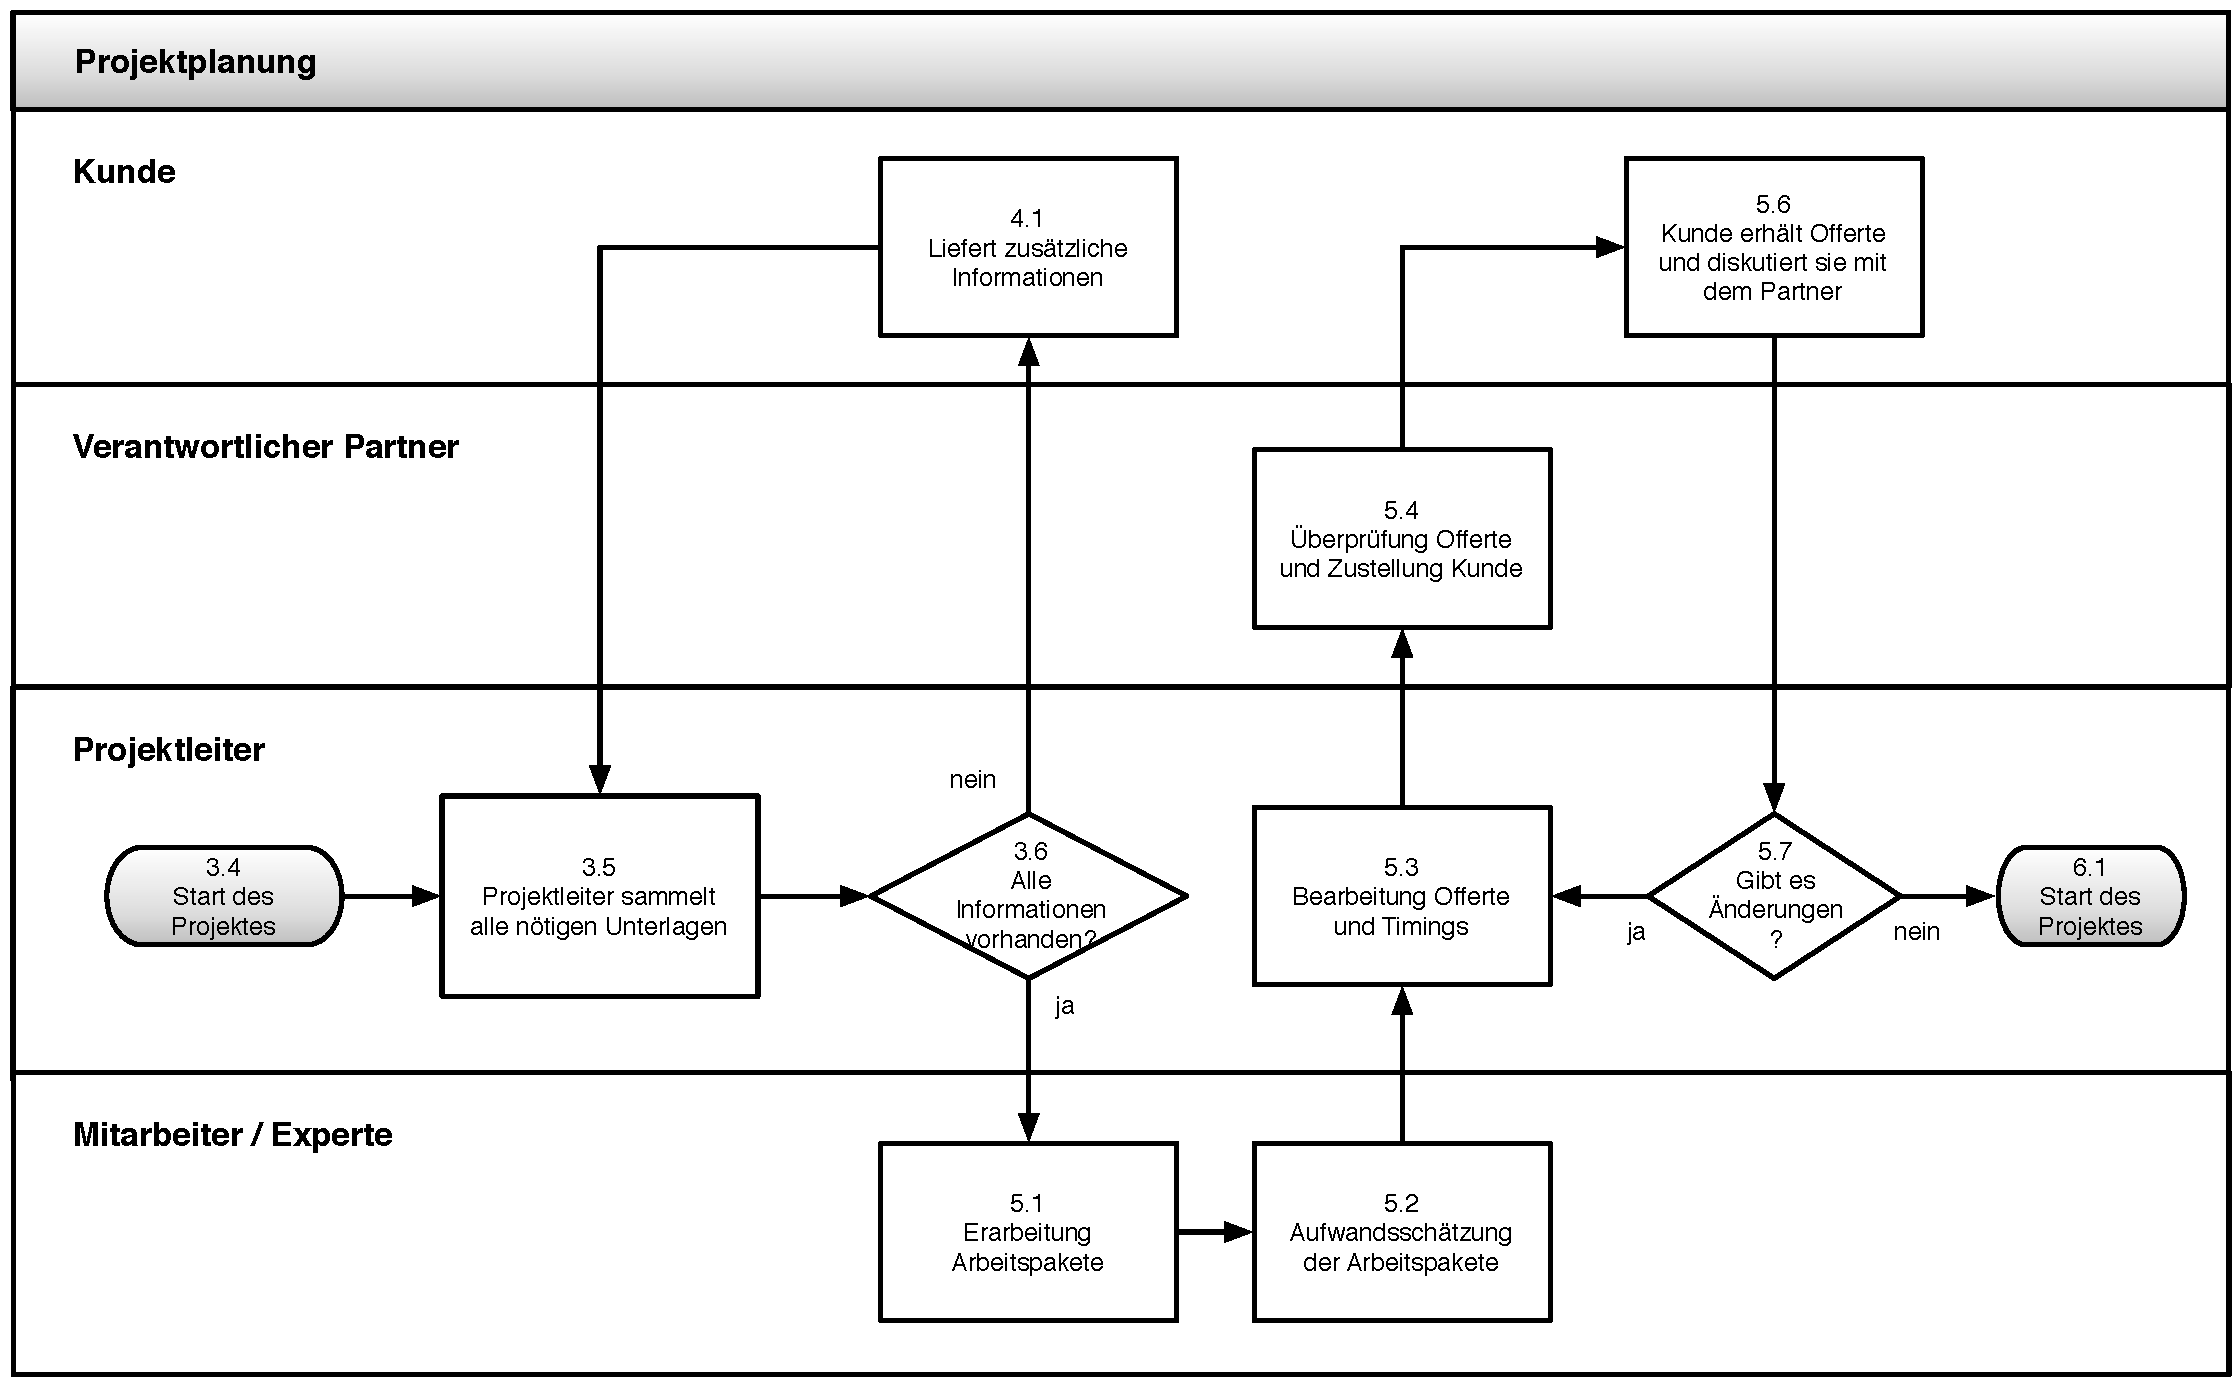
\includegraphics[width=0.99\textwidth,angle=0]{./bilder/loesung/02_02_projektplanung.pdf}
\caption[Ablauf der Projektplanungsphase]{Ablauf der Projektplanungsphase\footnotemark}
\label{pic:02_02_projektplanung}
\end{center}
\end{figure}
\footnotetext{Eigene Darstellung}

\subsubsection{Arbeitspakete}
Die in Zusammenarbeit mit den Mitarbeitern, Experten und, sofern nötig, mit dem
verantwortlichen Partner, erstellten Arbeitspakete werden vom Projektleiter
in Todo Listen im Projektmanagement Tool erfasst (\textbf{\addtocounter{icounter}{1}AI\arabic{icounter}}).
Wo sinnvoll und zu diesem Zeitpunkt schon offensichtlich ordnet er den Todos
auch schon die zuständigen Mitarbeiter zu.

\subsubsection{Aufwandsschätzung}
Dank dem Zuziehen der richtigen Mitarbeiter und Experten sollte die Aufwandsschätzung 
realistisch sein. Der zuständige Partner ist verantwortlich diese Schätzung
zu studieren und wenn nötig mit den dafür verantwortlichen Mitarbeitern zu 
diskutieren. Dies ist sehr wichtig, da auf der Aufwandsschätzung die Offerte 
und die Terminplanung basieren.

Zu diesem Zeitpunkt werden auch die nötigen Ressourcen geplant. Im Projektmanagement
Tool werden die nötigen Ressourcen reserviert (\textbf{\addtocounter{icounter}{1}AI\arabic{icounter}}). 
Falls es Konflikte in der Planung einzelner Mitarbeiter gibt, wird zuerst versucht 
einen anderen Mitarbeiter zu wählen. Falls dies nicht möglich ist entscheiden der 
Projektleiter und der verantwortliche Partner ob für dieses Projekt eine zusätzliche 
Ressource geschaffen werden soll, oder ob man eine Verzögerung des Projektes in Kauf 
nehmen kann. Dies hat einen Einfluss auf die parallel zu erstellende Terminplanung.

\subsubsection{Terminplanung}
Bei der Erstellung der Terminplanung ist es wichtig eine möglichst realistische
Zeitplanung zu erstellen. Diese ist nicht nur von der Aufwandsschätzung abhängig,
sondern kann auch von Kundenvorgaben oder Aufwänden von Drittanbietern beeinflusst
werden. Die erarbeiteten Meilensteine trägt der Projektleiter ebenfalls im
Projektmanagement Tool nach (\textbf{\addtocounter{icounter}{1}AI\arabic{icounter}})
und ordnet, wo sinnvoll, die erstellten Todo Listen den jeweiligen Meilensteinen
zu.

Zu diesem Zeitpunkt kann der Projektleiter auch die voraussichtlichen Geldflüsse planen.
Im Projektmanagement Tool erfasst er die genehmigten Offerten, externen Kosten
und Teilzahlungen bzw. Rechnungen (\textbf{\addtocounter{icounter}{1}AI\arabic{icounter}}).
Diese Informationen helfen der Geschäftsleitung eine projektübergreifende und
rollende Liquiditätsplanung zu erstellen.

\subsection{Projektkontrolle}
Während der Durchführung des Projektes kontrollieren der Projektleiter und der 
verantwortliche Partner laufend die Einhaltung der gesetzten Meilensteine und
geplanten Geldflüsse. Alle Mitarbeiter rapportieren während der Durchführung
täglich die aufgewendeten Stunden pro Projekt.

\subsubsection{Terminkontrolle}
Der Projektleiter behält die Abarbeitung der definierten Todo Listen und die
davon abhängigen Meilensteine im Auge. Sobald sich ein Verzug abzeichnet informiert
er frühzeitig den verantwortlichen Partner. In einer gemeinsamen Diskussion,
wenn nötig auch mit den Mitarbeitern des Projektes, wird das weitere Vorgehen
entschieden. Der Projektleiter oder verantwortliche Partner geht anschliessend
proaktiv auf den Kunden zu und informiert ihn über die Veränderungen. Der
Projektleiter passt die Planung im Projektmanagement Tool laufend an.

\subsubsection{Kostenkontrolle}
Der Projektleiter behält auch die auf sein Projekt rapportierten Stunden im Auge.
Er kontrolliert laufend, ob für Arbeiten mehr Stunden als geschätzt aufgewendet
wurden. Je nach Grösse der Abweichung informiert er den verantwortlichen
Partner, der wiederum das weitere Vorgehen entscheidet.

Der Projektleiter ist auch dafür verantwortlich, dass die geplanten Rechnungen
rechtzeitig gestellt werden. Die Geschäftsleitung kann diese projektübergreifend
im Projektmanagement Tool kontrollieren und bei Verzögerungen bei den jeweiligen
Projektleitern nachfragen.

\subsection{Projektabschluss}
Sobald alle Todos erledigt sind und alle Meilensteine erreicht wurden kommt
das Projekt in die Projektabschlusssphase. Diese ist in der Darstellung 
\ref{pic:02_03_projektabschluss} abgebildet. Als erstes kümmert sich der
Projektleitung darum, dass die Qualitätskontrolle durchgeführt wird (\textbf{7.2}). 
Sofern Mängel bemerkt werden (\textbf{7.3}), werden zusammen mit den Mitarbeitern zusätzliche
Arbeitspakete erstellt (\textbf{8.1}). Wurden keine Mängel entdeckt, erstellt
der Projektleiter den Produktabnahmebericht (\textbf{9.1}). Diesen bespricht er mit dem
verantwortlichen Partner. Dieser wiederum präsentiert dem Kunden die Resultate (\textbf{9.2})
und nimmt das Feedback nach dessen Begutachtung (\textbf{9.3}) entgegen (\textbf{9.4}).

Sind jetzt noch weitere Änderungen offen oder werden zusätzliche Änderungen
gewünscht (\textbf{9.5}), überprüft der Projektleiter zusammen mit dem verantwortlichen
Partner, ob die Anpassungen in den bereits gestellten Offerten enthalten sind, 
oder ob sie zusätzlich verrechnet werden können (\textbf{10.1}). Je nach Fall
passt er die Offerte an (\textbf{5.3}). So oder so werden zusammen mit den 
Mitarbeitern die zusätzlichen Arbeitspakete erstellt (\textbf{8.1}).

Wenn der Kunde vollständig mit dem Resultat zufrieden ist, schliesst der 
Projektleiter das Projekt ab (\textbf{11.1}). Dies beinhaltet das archivieren
aller Projektdaten (\textbf{\addtocounter{icounter}{1}AI\arabic{icounter}}), 
das nachführen des Projektstatus im Projektmanagement Tool und die Reflektionssitzung 
mit allen Projektmitarbeitern. Danach ist das Projekt beendet (\textbf{11.2}).

\clearpage

\begin{figure}[h!tbp]
\begin{center}
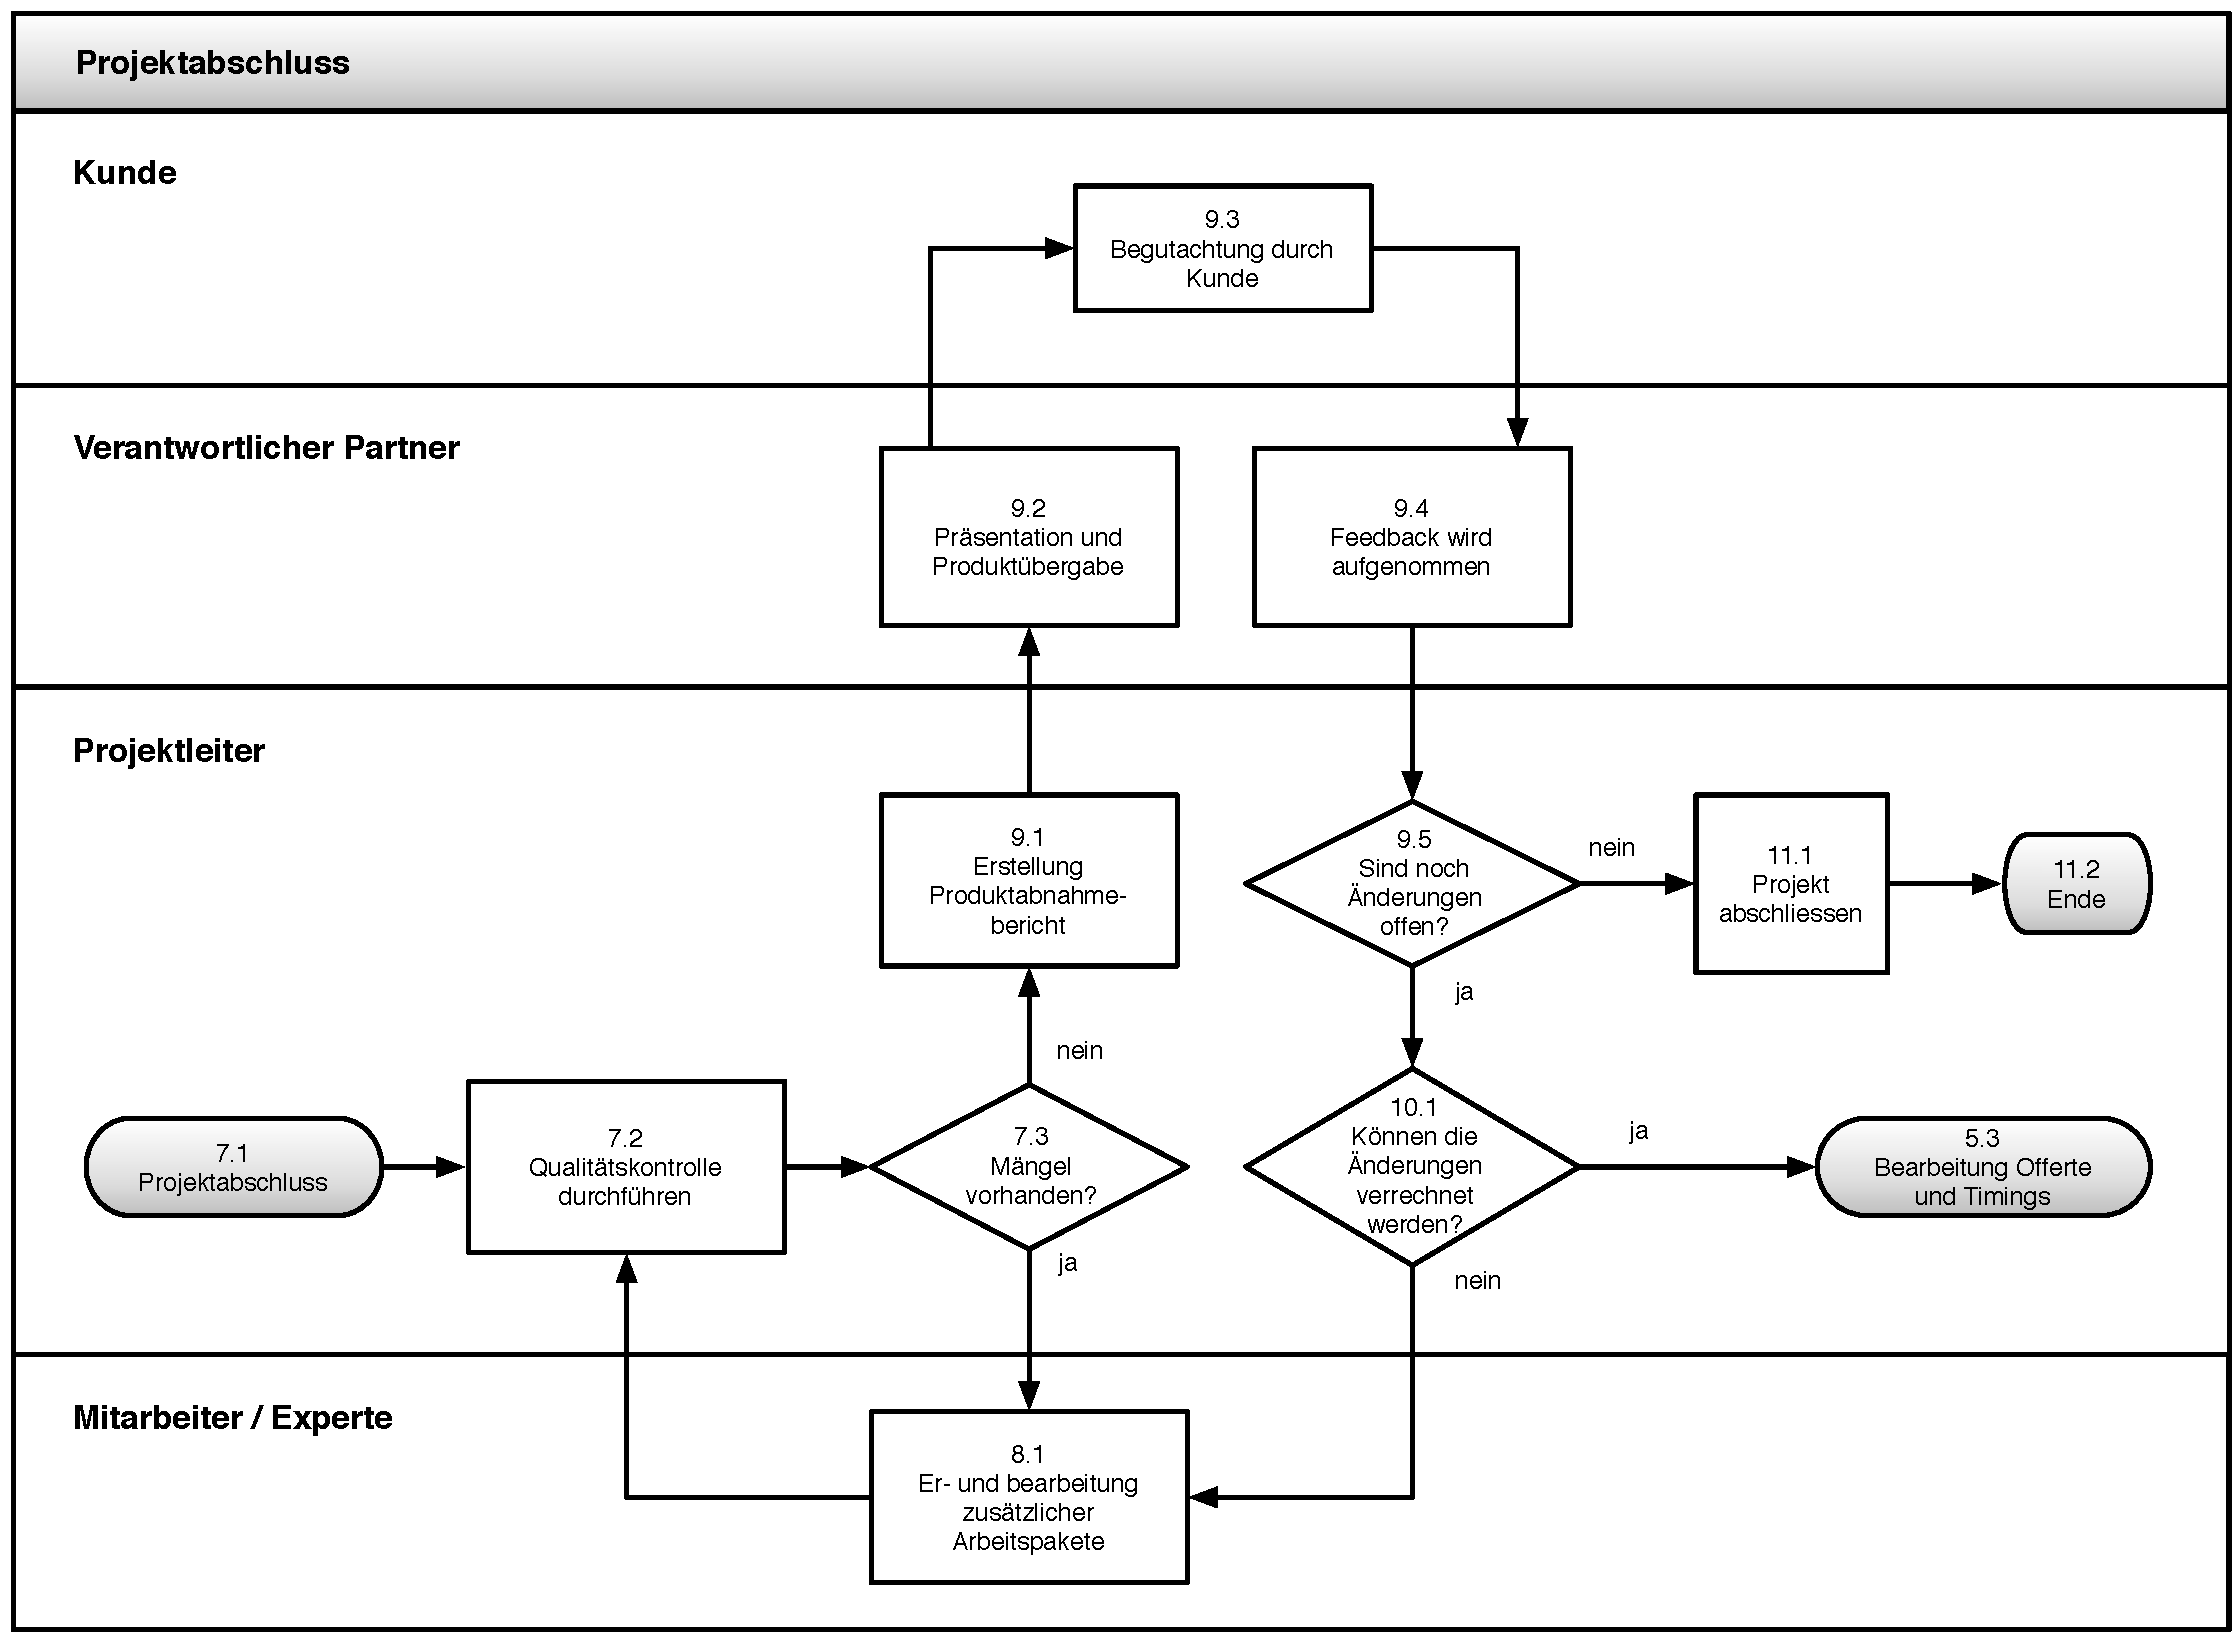
\includegraphics[width=0.99\textwidth,angle=0]{./bilder/loesung/02_03_projektabschluss.pdf}
\caption[Ablauf der Projektabschlusssphase]{Ablauf der Projektabschlusssphase\footnotemark}
\label{pic:02_03_projektabschluss}
\end{center}
\end{figure}
\footnotetext{Eigene Darstellung}

\clearpage

\subsubsection{Qualitätskontrolle}
Der Projektleiter organisiert in erster Linie die Qualitätskontrolle und sollte
sie nicht selbst durchführen, da er zu nahe am Projekt ist. Entweder übernimmt
dies der verantwortliche Partner oder ein aussenstehender Mitarbeiter.

\subsubsection{Produktabnahme}
Vor der Produktabnahme überprüft der Projektleiter noch einmal den Projektbrief
und alle Offerten. Die Resultate und sonstige Eigenheiten des Projektes hält er
in einem Produktabnahmebericht fest. Dieser bildet die Grundlage für die
Präsentation und Produktübergabe des verantwortlichen Partners und stellt
sicher, dass nichts vergessen gegangen ist.

\subsubsection{Reflektion}
An der Reflektionssitzung müssen alle Mitarbeiter des Projektes inklusive dem
verantwortlichen Partner, damit er die Resultate auch in die Geschäftsleitung 
tragen kann, anwesend sein. Alle positiven und negativen Erfahrungen des Projektes
werden diskutiert. Die Resultate müssen nicht zwingend festgehalten werden,
da die Diskussionen und somit die Verarbeitung der Erfahrungen im Vordergrund 
stehen.

\section{Instrumentenwahl}\label{chap:instrumentenwahl}
Im neuen Projektablauf des Lösungsansatzes wurde an diversen Stellen auf Instrumente
verwiesen, für die in diesem Kapitel noch die richtige Wahl getroffen werden
muss. Als erstes werden die einzelnen Verwendungen aufgelistet und beschrieben.
In einem weiteren Schritt werden verschiedene Varianten verglichen. Danach
kann die Geschäftsleitung der allink entscheiden, welche Instrumente sie
in Zukunft einsetzen möchte.

\subsection{Anforderungen aus dem Projektablauf}
In der nachfolgenden Tabelle \ref{tab:projektablauf_instrumente} sind alle
Anforderungen an die Instrumente, auf die im Projektablauf verwiesen wurde, aufgelistet 
und beschrieben.

\begin{longtable}{lp{14cm}}
    \toprule \textbf{Nr.} & \textbf{Beschreibung} \\
    \midrule AI1 & Ein Instrument, um ein neues Projekt zu eröffnen und um eine 
        eindeutige Projektnummer zu vergeben. \\
    \midrule AI2 & Ein Instrument, mit dem alle Projektmitarbeiter ihre 
        aufgewendeten Stunden rapportieren können. \\
    \midrule AI3 & Ein Instrument, um die Arbeitspakete bzw. Todos eines Projektes
        verwalten und überwachen zu können. \\
    \midrule AI4 & Ein Instrument, um die Ressourcenplanung erstellen zu können. \\
    \midrule AI5 & Ein Instrument, um die Meilensteine eines Projektes verwalten 
        und überwachen zu können.\\
    \midrule AI6 & Ein Instrument, um die Geldflüsse wie Offerten, Rechnungen 
        und Teilzahlungen verwalten und überwachen zu können. \\
    \midrule AI7 & Ein Instrument und Vorgaben, um alle Projektdaten archivieren 
        zu können. \\
    \bottomrule
    \caption[Im Projektablauf benötigte Instrumente]{Im Projektablauf benötigte 
        Instrumente\footnotemark}
    \label{tab:projektablauf_instrumente}
\end{longtable}
\footnotetext{Eigene Darstellung}

Es können natürlich mehrere Instrumente mit einer Variante abgedeckt werden.
Zum Beispiel mit der Projektmanagementsoftware Metronom\footnote{Metronom ist die 
Projektmanagementsoftware welche die FEINHEIT GmbH einsetzt.
Vgl. Kapitel \ref{chap:branchenvergleich}.}. Sie wurden jedoch absichtlich getrennt 
aufgelistet, damit für jedes Instrument verschieden Varianten aufgezeigt werden können.

\subsection{Instrumentenvergleich}
\newcounter{vcounter}
In der nachfolgenden Tabelle \ref{tab:instrumenten_varianten} sind alle
Instrumente, und somit alle möglichen Varianten die zur Auswahl stehen, aufgelistet 
und beschrieben. Die zur Auswahl stehenden Instrumente wurden zusammen mit der
Geschäftsleitung evaluiert.

Natürlich gibt es diverse weitere Produkte um diese
Anforderungen abdecken zu können. Diese wurden aber zusammen mit der Geschäftsleitung
der allink beschränkt, da zum Beispiel eine SAP-Lösung\footnote{SAP bietet angepasste
Softwarelösungen für sämtliche Geschäftsprozesse eines Unternehmens.} gar 
nicht in Frage kommen würde und somit nicht weiter betrachtet werden muss.
Auch fällt eine vollständige Eigenentwicklung weg, da allink sich in Zukunft nicht
um die Pflege eines ganzen Projektmanagement Systems kümmern möchte. Erweiterungen
bestehender Systeme werden aber in Betracht gezogen, sofern die Systeme dies
ermöglichen.

\clearpage

Im Fokus stehen nun noch die Projektmanagement Software Metronom und Basecamp\footnote{Basecamp
ist eine webbasierte Projektmanagement Software von 37signals, \url{http://basecamphq.com/}}.
Die API\footnote{Eine API ist eine Programmierschnittstelle, die ein System zur Verfügung 
stellt um anderen Systemen die darin verwalteten Informationen zugänglich zu machen.} 
von Basecamp zur Anbindung weiterer Software ist zudem für eigene Erweiterungen 
sehr interessant.

\begin{longtable}{lllp{8cm}}
    \toprule
    \textbf{Anf.} & \textbf{Nr.} & \textbf{Instrument} & \textbf{Beschreibung} \\
    
    \midrule AI1 
    & \addtocounter{vcounter}{1}I\arabic{vcounter} & Metronom & Die webbasierte 
        Projektmanagement Software Metronom bietet eine Projektverwaltung an. \\
    & \addtocounter{vcounter}{1}I\arabic{vcounter} & Basecamp & Die ebenfalls 
        webbasierte Projektmanagement Software Basecamp
        bietet auch eine Projektverwaltung an. \\
    
    \midrule AI2 
    & \addtocounter{vcounter}{1}I\arabic{vcounter} & Metronom & Metronom bietet 
        die Möglichkeit Zeit auf sogenannte Tickets zu rapportieren. \\
    & \addtocounter{vcounter}{1}I\arabic{vcounter} & Basecamp & Basecamp bietet
        ebenfalls die Möglichkeit Zeit auf ein Projekt oder Todo zu rapportieren. \\
    & \addtocounter{vcounter}{1}I\arabic{vcounter} & Basecamp Erweiterung & Dank
        der API von Basecamp könnte eine kleine Software entwickelt werden, die
        das Rapportieren dem Mitarbeiter so einfach wie möglich macht, jedoch
        die Daten weiterhin im Basecamp ablegt. \\
    
    \midrule AI3
    & \addtocounter{vcounter}{1}I\arabic{vcounter} & Metronom & Mit Metronom können
        die laufenden Arbeitspakete und Tickets eines Projektes verwaltet und
        überwacht werden. \\
    & \addtocounter{vcounter}{1}I\arabic{vcounter} & Basecamp & Basecamp bietet
        ebenfalls das Verwalten und Überwachen von Arbeitspaketen und Todos an. \\
    
    \midrule AI4 
    & \addtocounter{vcounter}{1}I\arabic{vcounter} & Metronom & Metronom ermöglicht
        nur eine beschränkte Ressourcenplanung. Man kann die Summe aller geplanten
        Tickets pro Mitarbeiter auswerten. \\
    & \addtocounter{vcounter}{1}I\arabic{vcounter} & Excel & Die Ressourcenplanung
        könnte auch in einem Microsoft Excel oder Apple Numbers File geführt werden. \\
    & \addtocounter{vcounter}{1}I\arabic{vcounter} & Eigenentwicklung & Für die
        Ressourcenplanung könnte allink eine eigene Software mit Fokus auf
        ihre Bedürfnisse entwickeln und ebenfalls an z.B. Basecamp koppeln. \\
    
    \midrule AI5 
    & \addtocounter{vcounter}{1}I\arabic{vcounter} & Metronom & Mit Metronom
        können Meilensteine geplant und verwaltet werden. \\
    & \addtocounter{vcounter}{1}I\arabic{vcounter} & Basecamp & Auch Basecamp
        bietet die Möglichkeit, Meilensteine zu planen und zu verwalten.\\
    
    \midrule AI6 
    & \addtocounter{vcounter}{1}I\arabic{vcounter} & Metronom & Metronom bietet
        auch hier alle nötigen Funktionen um die Geldflüsse zu planen. Jedoch
        ist die Software bei der Darstellung von den Übersichten und Rechnungen
        sehr eingeschränkt. \\
    & \addtocounter{vcounter}{1}I\arabic{vcounter} & Eigenentwicklung & Hier
        könnte allink ebenfalls eine eigene Software mit Anbindung an
        Basecamp entwickeln, um genau ihre Bedürfnisse abdecken zu können.\\
    
    \midrule AI7 
    & \addtocounter{vcounter}{1}I\arabic{vcounter} & allink Server & Hier kann
        der schon vorhandene Fileserver von allink eingesetzt werden.\\
    
    \bottomrule
    \caption[Zur Auswahl stehende Varianten der Instrumente]{Zur Auswahl stehende 
        Varianten der Instrumente\footnotemark}
    \label{tab:instrumenten_varianten}
\end{longtable}
\footnotetext{Eigene Darstellung}

\subsection{Variantenentscheid}
Obwohl Metronom bei der Auflistung der Varianten öfters gewählt werden könnte,
hinterlässt die Software beim Testen einen eher schwerfälligen Eindruck.
Basecamp wurde von allink schon öfters in Projekten mit anderen Agenturen 
verwendet und hat bis jetzt nur Anklang gefunden.

Nach längeren Diskussionen mit der Geschäftsleitung entscheidet sich die allink
für die Projektmanagement Software Basecamp und die Umsetzung von eigenen Erweiterungen. So muss
sich allink nicht um den Kern der Software kümmern und kann für ihre Bedürfnisse
passende Erweiterungen entwickeln. Somit wurde entschieden, die Instrumente I2,
I5, I7, I10, I12, I14 und I15 einzusetzen. In der nachfolgenden Abbildung \ref{pic:04_systemlandschaft} 
ist die neu geplante Systemlandschaft des Projektmanagements skizziert.

\begin{figure}[htbp]
\begin{center}
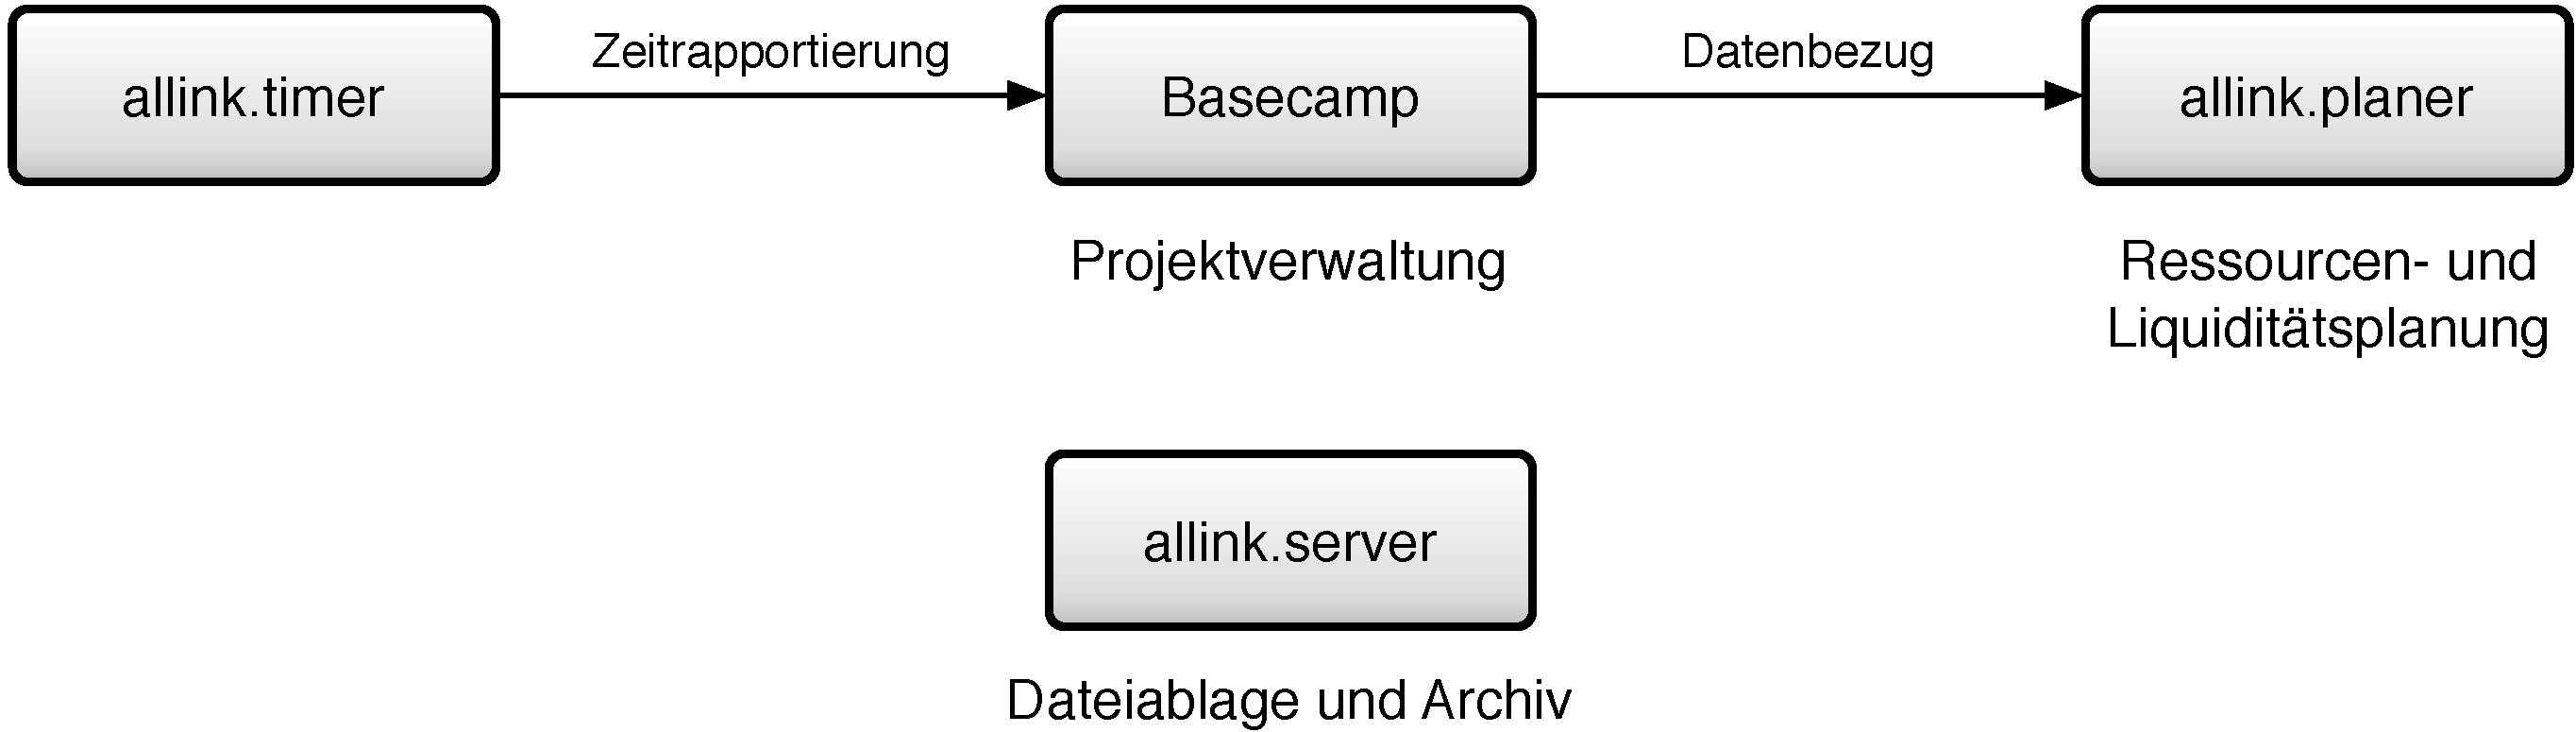
\includegraphics[width=0.8\textwidth,angle=0]{./bilder/loesung/04_systemlandschaft.pdf}
\caption[Neu geplante Systemlandschaft des Projektmanagements]{Neu geplante 
    Systemlandschaft des Projektmanagements\footnotemark}
\label{pic:04_systemlandschaft}
\end{center}
\end{figure}
\footnotetext{Eigene Darstellung}

Nachfolgend wird auf die einzelnen Elemente der neuen Systemlandschaft
eingegangen und jeweils auf die erfüllende Anforderung aus dem neuen Projektablauf
verwiesen.

\subsubsection{Basecamp}
Als zentrales Element dient neu die kostenpflichtige Projektmanagement Software 
Basecamp zur Erfassung und Verwaltung der Projekte (\textbf{AI1}). Darin werden alle
Arbeitspakete, Todos, Meilensteine und die rapportierten Stunden geführt (\textbf{AI3} 
und \textbf{AI5}). Basecamp bietet, wie bereits erwähnt, eine Schnittstelle um
andere Systeme anzubinden. Diese wird in den zwei nachfolgenden Eigenentwicklungen
genutzt.

\subsubsection{allink.timer}
Es wird eine kleine Software namens allink.timer entwickelt, worüber Mitarbeiter 
möglichst einfach ihre Stunden pro Projekt rapportieren können (\textbf{AI2}). 
Diese Software bezieht die laufenden Projekte aus Basecamp und speichert die 
rapportierten Stunden wieder zurück.

\subsubsection{allink.planer}
Für die Ressourcenplanung und die Planung der Geldfüsse wird zusätzlich eine 
Software names allink.planer entwickelt. Darin werden alle Ressourcen, Offerten, 
Rechnungen und Teilzahlungen verwaltet und überwacht (\textbf{AI4} und \textbf{AI6}).
Es wurde bereits jetzt über eine zukünftige Erweiterung diskutiert, um 
Offerten und Rechnungen direkt aus dieser Software generieren zu können.

\subsubsection{allink.server}
Für die Ablage und Archivierung der Projektdaten wird der schon vorhandene
allink Server verwendet (\textbf{AI7}). Alle Mitarbeiter werden Zugriff auf die Unterlagen
von laufenden wie auch archivierte Projekten haben. Die Projektstruktur
wurde zusammen mit der Geschäftsleitung definiert und soll für laufende
wie auch archivierte Projekte, wie in der folgenden Abbildung \ref{pic:05_ablagestruktur} 
dargestellt, aufgebaut sein.

\begin{figure}[htbp]
\begin{center}
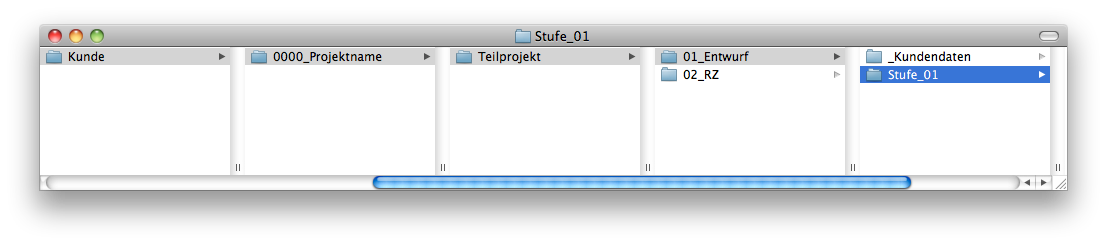
\includegraphics[width=1.0\textwidth,angle=0]{./bilder/loesung/05_ablagestruktur.png}
\caption[Ablagestruktur laufender und archivierter Projekte]{Ablagestruktur 
    laufender und archivierter Projekte\footnotemark}
\label{pic:05_ablagestruktur}
\end{center}
\end{figure}
\footnotetext{Eigene Darstellung}

Pro Kunde existiert ein mit dem Namen des Kunden beschrifteten Ordner. Darin befindet
sich pro Projekt jeweils ein Ordner mit genauer Projektbezeichnung inklusive Projektnummer.
Darin kann, sofern notwendig, noch in Teilprojekte unterschieden und
pro Teilprojekt ein Ordner erstellt werden. Im Projekt- oder Teilprojektordner
existieren im Minimum ein Ordner ``01 Entwurf'' und ``02 RZ'', wobei RZ für Reinzeichnung
steht. Im Reinzeichnungsordner werden die am Ende verwendeten Dateien abgelegt.
In den Entwurfsordner werden Kundendaten und die verschiedenen Stufen der Entwürfe
abgelegt.

\subsection{Überblick der Softwareveränderung}
Durch den Entscheid, welche Software in Zukunft im Projektmanagement eingesetzt
wird, verändert sich die Softwarelandschaft bei allink. In der nachfolgenden
Tabelle \ref{tab:neu_verwendete_software} wird alle Software aufgelistet, die 
bisher eingesetzt wurde\footnote{Vgl. Kapitel \ref{chap:verwendete_software}} 
und neu eingekauft oder entwickelt wird.

\newcounter{scounter}
\begin{longtable}{lllll}
    \toprule \textbf{Nr.} & \textbf{Bezeichnung} & \textbf{Hersteller} & \textbf{Kategorie} & \textbf{Status} \\
    \midrule \addtocounter{scounter}{1}S\arabic{scounter} & MacOS X & Apple & 
        Betriebssystem & wird beibehalten \\
    \midrule \addtocounter{scounter}{1}S\arabic{scounter} & Microsoft Windows & 
        Microsof & Betriebssystem & wird beibehalten \\
    \midrule \addtocounter{scounter}{1}S\arabic{scounter} & MacOS X Server & Apple & 
        Betriebssystem & wird beibehalten \\
    \midrule \addtocounter{scounter}{1}S\arabic{scounter} & Apple iWork & Apple & 
        Office Suite & wird beibehalten \\
    \midrule \addtocounter{scounter}{1}S\arabic{scounter} & Microsoft Office & 
        Microsoft & Office Suite & wird beibehalten \\
    \midrule \addtocounter{scounter}{1}S\arabic{scounter} & Apple Mail & Apple & 
        E-Mail Software & wird beibehalten \\
    \midrule \addtocounter{scounter}{1}S\arabic{scounter} & Stundenwidget & allink & 
        Dashboardwidget & wird abgelöst \\
    \midrule \addtocounter{scounter}{1}S\arabic{scounter} & Basecamp & 37signals & 
        Projektmanagement & wird eingekauft \\
    \midrule \addtocounter{scounter}{1}S\arabic{scounter} & allink.timer & allink & 
        Projektmanagement & wird entwickelt \\
    \midrule \addtocounter{scounter}{1}S\arabic{scounter} & allink.planer & allink & 
        Projektmanagement & wird entwickelt \\
    \bottomrule
    \caption[Neue Softwarelandschaft bei allink]{Neue Softwarelandschaft bei allink\footnotemark}
    \label{tab:neu_verwendete_software}
\end{longtable}
\footnotetext{Eigene Darstellung}

Die Software Basecamp wurde nach der Entscheidung von allink eingekauft.
Mit der Entwicklung der Projektmanagement Tools allink.timer und allink.planer
wurde bereits begonnen. Der Studierende hat zwei funktionierende Prototypen 
erstellt. Da die Softwareentwicklung nicht Bestandteil dieser Arbeit ist, wird
auf eine ausführliche Dokumentation verzichtet. Sie werden jedoch im ``Proof of
Concept'' im Kapitel \ref{chap:proof_of_concept} zur Anwendung kommen.


\section{Anforderungsabdeckung}
Da der Lösungsansatz mit dem neuen Projektablauf und der Wahl der Instrumente
abgeschlossen ist, muss noch überprüft werden, ob die Anforderungen an den
neuen Projektablauf abgedeckt werden konnten.

Dazu werden die im Kapitel \ref{chap:akzeptanzkriterien} definierten 
Akzeptanzkriterien durchlaufen und geprüft. Dies ist in der nachfolgenden Tabelle 
\ref{tab:akzeptanzkriterien_test} ersichtlich. Zur besseren Lesbarkeit wurde zur 
Akzeptanzkriteriumsnummer das Kriterium ein weiteres mal aufgelistet. Dazu wird 
der Status der Erfüllung gezeigt und in kurzen Worten beschrieben, wodurch das
Kriterium erfüllt wird.

\begin{longtable}{lp{6cm}p{5cm}l}
    \toprule \textbf{Nr.} & \textbf{Kriterium} & \textbf{Beschreibung} & \textbf{Status} \\
    \midrule AK1 &
        Wurde für das Projekt ein Hauptverantwortlicher Projektleiter definiert? &
        In der Projektdefinitionsphase Schritt 3.1. &
        erfüllt \\
    \midrule AK2 &
        Wurde für das Projekt ein Hauptverantwortlicher Partner definiert? &
        In der Projektdefinitionsphase Schritt 3.1 &
        erfüllt \\
    \midrule AK3 &
        Existiert für das Projekt ein Projektbrief? &
        In der Projektdefinitionsphase Schritt 3.2 &
        erfüllt \\
    \midrule AK4 &
        Können für das Projekt Meilensteine und Arbeitspakete definiert werden? &
        Mit der Software S8 &
        erfüllt \\
    \midrule AK5 &
        Können die Mitarbeiter auf das Projekt Stunden rapportieren? &
        Mit der Software S9 &
        erfüllt \\
    \midrule AK6 &
        Sind die definierten Projektkennzahlen in einem System ersichtlich? &
        Mit der Software S10 &
        erfüllt \\
    \midrule AK7 &
        Sind die definierten Liquiditäts-Kennzahlen in einem System ersichtlich? &
        Mit der Software S10 &
        erfüllt \\
    \midrule AK8 &
        Existiert eine klare Struktur zur Ablage der Projektdaten? &
        Wurde Projektübergreifend definiert, Abbildung \ref{pic:05_ablagestruktur} &
        erfüllt \\
    \midrule AK9 &
        Wurde für das Projekt ein Hauptverantwortlicher für die Qualitätssicherung definiert? &
        In der Projektabschlussphase Schritt 7.2 &
        erfüllt \\
    \bottomrule
    \caption[Überprüfung der Akzeptanzkriterien der definierten Anforderungen]{Überprüfung 
        der Akzeptanzkriterien der definierten Anforderungen\footnotemark}
    \label{tab:akzeptanzkriterien_test}
\end{longtable}
\footnotetext{Eigene Darstellung}

Es wurden alle Akzeptanzkriterien erfüllt. Ob nun der in der Theorie geplante
Lösungsansatz auch in der Praxis umgesetzt werden kann und die Akzeptanzkriterien
in der Realität auch tatsächlich erfüllt werden, wird der im nächsten und
letzten Kapitel durchgespielte ``Proof of Concept'' zeigen.
